\documentclass[a4paper]{ctexrep}
\usepackage{mathtools}
\usepackage{tikz}
\usepackage{chemfig}
\usepackage[version=4]{mhchem}
\usepackage{float}


\author{Y.C. Long}
\title{有机化学 -- 孙净雪}


\begin{document}
    \maketitle
    \tableofcontents
    

    % 孙净雪 - 13384608260
    % 期末闭卷70分,出勤10分,课堂小测验10分,作业10分。作业交了就行。
    % 老师是两批老师,所以这个课会用一点时间过渡一下
    \chapter*{学期过渡部分}
    \section*{基本反应回顾}
    \begin{itemize}
        \item 烷烃--自由基引发,取代
        \item 烯烃--加成,亲电,$\pi$电子云是裸露在外的
        \item P--X 卤代烃 没有不饱和度,被亲核试剂进攻
        \item 芳烃 亲电试剂进攻
    \end{itemize}

    \section*{亲核试剂和亲电试剂}
    
    \subsection*{亲电试剂}

    \begin{enumerate}
        \item 单质 $\ce{X2}$
        \item 强酸 $\ce{HCl}$
        \item 缺电子化物 
    \end{enumerate}

    \subsection*{亲核试剂}

    \begin{enumerate}
        \item 弱酸、弱酸眼 $\ce{HCN}$,$\ce{NaCN}$
        \item 含有未成键电子对化合物 $\ce{NH3}$
        \item 格氏试剂 $\ce{RMgX}$
    \end{enumerate}

    \chapter{酚}
\section{概述}
酚(phenols, $\ce{Ar-OH}$)
羟基直接与苯环\textit{$sp^2$}碳原子相连接的化合物称为酚,苯酚(\scalebox{0.6}[0.6]{\chemfig{OH-[:180,,1]=_[:240]-[:180]=_[:120]-[:60]=_(-[:300])}})最为常见,另外还有萘酚等。

\subsection{分类}
\begin{enumerate}
    \item 芳环类型
    \item $\ce{-OH}$的个数
\end{enumerate}
\subsection{命名}
不考,没啥用,知道大概啥顺序就行

\section{物理性质}
\begin{enumerate}
    \item 形成分子间氢键,沸点较高
    \item 对称性较好,熔点较高,常温下是固体
    \item 水溶性 苯酚在冷水中微溶,加热时可以无限溶解 \par
    与醇相比,苯酚和水形成氢键的能力比较差。($sp^3$和$sp^2$)\footnote{$sp^3$杂化距离更远,跟适合形成氢键。酚只有一对$sp^2$电子,比醇还少一对}
    \item 酚本身无色,容易被空气中的氧气氧化而略呈红色或褐色
    \item 有毒
\end{enumerate}

\section{化学性质}
\subsection{$\ce{C-O}$ 键}
不容易断。酚具有一定的离域,具有一定的双键性质。

\subsection{$\ce{O-H}$ 键}
\begin{enumerate}
    \item 酸性
    \item 含有未成对的电子---碱性、亲核性
    \item 配位性,可以和铁发生显色反应
\end{enumerate}

\subsection{苯环}
\begin{enumerate}
    \item 亲电取代,$\ce{-OH}$是邻对位定位基,可以使苯环活化
    \item 氧化(复杂,机理不甚明确)
\end{enumerate}

\subsection{酚的酸性}

\subsubsection{不同类}
$\ce{H2CO3} > \ce{Ph-OH} > \ce{H2O} > \ce{ROH}$

若芳香基团上有吸电子基团,则酚酸性增强

\subsubsection{同类}

\begin{enumerate}
    \item 吸电子基 酸性增加 \par
    \begin{figure}[H]
        \scriptsize
        \centering
        \chemfig{*6(=-=-(-OH)=-)} < \chemfig{*6(=-(-NO_2)=-(-OH)=-)} < \chemfig{*6(=(-NO_2)-=-(-OH)=-)}
    \end{figure}
    \item 供电子基 酸性降低 \par
    \begin{figure}[H]   
        \scriptsize
        \centering
        \chemfig{*6(=-=-(-OH)=-)} < \chemfig{*6(=-(-CH_3)=-(-OH)=-)} < \chemfig{*6(=(-CH_3)-=-(-OH)=-)}
    \end{figure}
    \item 卤素 吸电子,酸性增加
\end{enumerate}

\subsection{显色反应}
可以与铁形成紫色复合物

$\ce{6C6H6OH + FeCl3 -> H_3[Fe(OC6H5)] + 3HCl}$

\subsection{亲核性}

亲核性 只和易发生亲核反应的物质反应

如 
\begin{figure}[H]
    \scriptsize
    \centering
    \schemestart
    \chemfig{R-C(=[:90]O)-Cl} \+ \chemfig{*6(-=-=(-OH)-=)} \arrow
    \schemestop
\end{figure}

\subsection{亲电取代}

\subsubsection{卤代反应}

\begin{figure}[H]
    \scriptsize
    \centering
    \schemestart
    \chemfig{*6(-=-=(-OH)-=)}  \+ $\ce{Br2}$ \arrow \chemfig{*6(-(-Br)=-(-Br)=(-OH)-(-Br)=)}
    \schemestop
\end{figure}
原因:水中存在 \scriptsize\chemfig{*6(-=-=(-{O^{-}})-=)}\normalsize,要想控制反应进度,可以在有机溶剂中进行:

\begin{figure}[H]
    \scriptsize
    \centering
    \schemestart
    \chemfig{*6(-=-=(-OH)-=)} \arrow{->[$\ce{Br}$][$\ce{CS2}, 0^\circ \mathrm{C}$]} \chemfig{*6(-(-Br)=-=(-OH)-=)} + \chemfig{*6(-=-(-Br)=(-OH)-=)}
    \schemestop
\end{figure}

\subsubsection{磺化反应}

\begin{figure}[H]
    \scriptsize
    \centering
    \schemestart
    \chemfig{*6(-=-=(-OH)-=)} \+ $\ce{H2SO4}$ \arrow \chemfig{*6(-=-(-SO_3)=(-OH)-=)} \+ \chemfig{*6(-(-SO_3)=-=(-OH)-=)}
    \schemestop
\end{figure}
\subsubsection{硝化反应}

一般来讲不要直接硝化,不然产率会很低

\begin{figure}[H]
    \scriptsize
    \centering
    \schemestart
    \chemfig{*6(-=-=(-OH)-=)} \arrow{->[$\ce{NaNO2}$][$\ce{H+}$]} \chemfig{*6(-(-NO)=-=(-OH)-=)} \arrow{->[$\ce{HNO3}$]} \chemfig{*6(-(-NO_2)=-=(-OH)-=)}
    \schemestop
\end{figure}

\subsubsection{傅氏反应}

\begin{figure}[H]
    \scriptsize
    \centering
    \schemestart
    \chemfig{*6(-=-=(-OH)-=)} \+ $\ce{RCl}$ \arrow{->[HF]} \chemfig{*6(-(-R)=-=(-OH)-=)}
    \schemestop
\end{figure}

\subsubsection{氧化反应}

\begin{figure}[H]
    \scriptsize
    \centering
    \schemestart
    \chemfig{*6(-=-=-=)} \arrow{->[$\mbox{[O]}$]} \chemfig{*6(-(=O)-=-(=O)-=)}
    \schemestop
\end{figure}

\subsection{酚的制法(了解)}



    \chapter{醛、酮}

    
    \section{概述}

    \subsection{分类}

    \begin{enumerate}
        \item 脂肪型
        \item 芳香型
    \end{enumerate}

    \subsection{羰基的结构特点 -- 极性不饱和基团}

    碳和氧都采用$sp^2$杂化,碳氧双键中,成键电子云分布不均匀,而是偏向氧原子。

    \section{物理性质}


\subsection{酰卤}

\begin{center}
    \chemfig{R-[:30]C(=[:90]O)-[:-30]X}
\end{center}

不能形成分子间的氢键。

\subsection{酯、酸酐}

\begin{center}
    \chemfig{R-[:30]C(=[:90]O)-[:-30]OR}
\end{center}

\begin{center}
    \chemfig{R-[:30]C(=[:90]O)-[:-30]O-[:30]C(=[:90]O)-[:-30]R}
\end{center}

也不能形成氢键,低级酯一般为液体,高级酯一般为固体。
    \section{化学性质}

\subsection{通性}


\begin{enumerate}
    \item 羧酸有酸性(有相对来说比较弱的亲核性)
    \item 亲核取代反应(生成羧酸衍生物)
    \item 羧酸是比较高的氧化态,可以被还原
    \item 受到羰基的影响,碳氢键也可能发生一些$\alpha - \ce{H}$异裂的反应。
    \item 脱羧反应
\end{enumerate}


\subsection{酸性}

羧酸的酸性是一种弱酸,比碳酸强。羧酸与无机酸的酸性比较:

\[
    \ce{HCl} > \ce{CH3COOH} > \ce{H2CO3}  
\]

吸电子诱导效应会导致羧酸的酸性增强。供电子诱导效应会导致羧酸的酸性减弱。

\[
    \ce{Ph-COOH} > \ce{CH3COOH}  
\]

供电子效应\scriptsize \chemfig{*6(-=-=-=)}\normalsize 比\chemfig{-[,0.5]CH_3}强


\subsection{亲核取代反应}

\subsubsection{合成酰卤$\ce{SOCl2}$、$\ce{PCl3}$}


\begin{center}
    \scriptsize
    \schemestart
    \chemfig{RCOOH} \+ $\ce{SOCl2}$ \arrow  \chemfig{R-C(=[:90]O)-Cl}
    \schemestop
\end{center}

\subsubsection{合成酸酐}

一般使用$\ce{P2O5}$。酸酐分为``外酸酐''和``内酸酐'',内酸酐主要是分子内脱水形成的酸酐。``外酸酐''可以自己和自己脱水形成酸酐,甚至可以两种不同的羧酸脱水形成``混酸酐''。

\begin{center}
    \scriptsize
    \schemestart
    \chemfig{RCOOH} \+ $\ce{SOCl2}$ \arrow  \chemfig{R-C(=[:90]O)-Cl}
    \schemestop
\end{center}


内酸酐

\begin{center}
    \scriptsize
    \schemestart
    \chemfig{*6(-=(-COOH)-(-COOH)=-=)} \+ \arrow{->[$\Delta$][$\ce{P2O5}$]}[,1.3] \chemfig{*6(-=(-C(=[:-90]O)-[:60]O?)-(-C?(=[:90]O))=-=)}
    \schemestop
\end{center}


要合成混酸酐,需要使用酰卤和酸盐来合成。

\begin{center}
    \scriptsize
    \schemestart
    \chemfig{R-[:30]C(=[:90]O)-[:-30]ONa} \+ \chemfig{Cl-[:30]C(=[:90]O)-[:-30]\textbf{R} } \arrow  \chemfig{R-[:30]C(=[:90]O)-[:-30]O-[:30]C(=[:90]O)-[:-30]\textbf{R}}
    \schemestop
\end{center}


\subsubsection{合成酯}

高中学过的反应,与醇脱水形成酯。羧酸和醇在酸催化下加热失水生成的化合物称为酯(ester)。酯化反应是可逆反应。酸脱羟基、醇脱氢比较常见,也有一些反应相反,取决于反应的历程。

\begin{center}
    \scriptsize
    \schemestart
    \chemfig{RCOOH} + $\ce{ROH}$ \arrow{->} \chemfig{R-C(=[:90]O)-OR}
    \schemestop
\end{center}


\begin{center}
    \scriptsize
    \schemestart
    \chemfig{R-C(=[:90]O)-OH} \arrow{<=>[$\ce{H+}$]} \chemfig{R-C(=[:90]O\charge{75=+}{H})-OH} \arrow{->[$\ce{ROH}$]}
    \schemestop
\end{center}

但也有少数酯化反应中,酸或醇的羟基质子化,水离去,生成酰基正离子或碳正离子中间体,该中间体再与醇或酸反应生成酯。这些反应不遵循``酸出羟基醇出氢''的规则。

\begin{figure}[H]
    \centering
    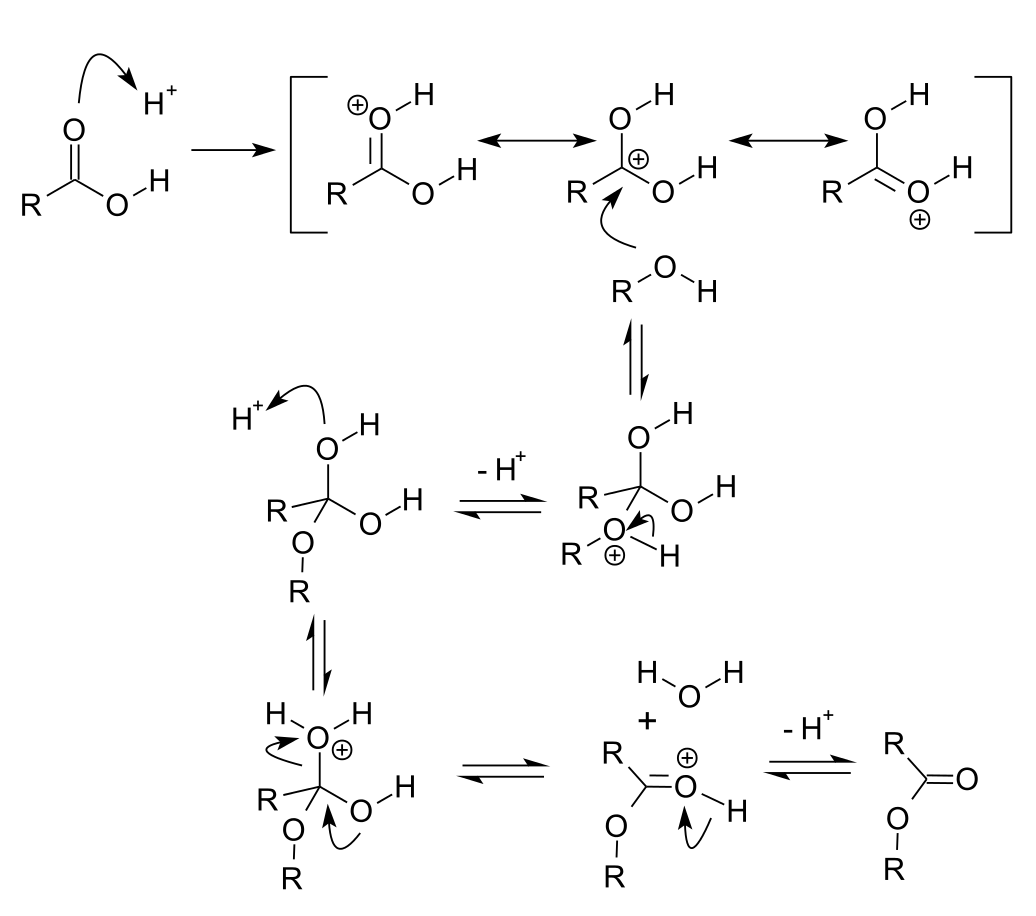
\includegraphics[width=0.7\textwidth]{img/Fischer_esterification_mechanism.png}
\end{figure}

\subsubsection{酰胺}

\begin{center}
    \scriptsize
    \schemestart
    \chemfig{RCOOH} + $\ce{NH3}$ \arrow{->} \chemfig{R-C(=[:90]O)-NH_2}
    \schemestop
\end{center}

\subsection{还原反应}

被氢化铝锂还原为醇。

\subsection{脱羧反应}

条件:$\alpha$-C上有强吸电子基团


\subsection{$\alpha$-H取代反应}


HVZ 反应,红磷催化下,脂肪酸$\alpha$碳原子上的氢可以被卤素取代而生成$\alpha$卤代酸。

\begin{center}
    \scriptsize
    \schemestart
    \chemfig{R-CH_2-COOH} + $\ce{Br2}$ \arrow{->[P]} \chemfig{R-CH(-[:90]Br)-COOH} \arrow{->[\ch{H2O}]} \chemfig{R-CH(-[:90]OH)-COOH}
    \schemestop
\end{center}

\begin{reaction*}
    P + Br2 -> PBr3
\end{reaction*}

    
    \section{不饱和的醛或者酮}

    不饱和羰基化合物,就是分子中除了羰基外,还含有不饱和键的化合物。一般来说是指$\alpha, \beta$不饱和醛酮,这些化合物具有共轭的性质。最简单的$\alpha, \beta$ 不饱和醛酮是丁烯酮。

    \begin{center}
        \schemestart
        \chemname{\chemfig{=[:-30]-[:30](=[:90]O)-[:-30]}}{丁烯酮}
        \schemestop
    \end{center}

    \subsection{$\alpha, \beta$ 不饱和醛酮}

    $\ce{C=C}$上可以亲电加成$\ce{C=O}$上可以亲核加成。

    \subsubsection{氧化反应}

    弱氧化剂下,将醛氧化为羧酸(盐)。强氧化剂下,将双键和醛基都氧化,生成两种羧酸(或进一步反应)。

    \subsubsection{还原反应}

    如果是$\ce{NaBH4}$ 双键不变,将醛还原成醇(可以得到烯醇)。如果是催化加氢,则还原为饱和的醇。

    \subsubsection{双烯合成反应}

    $\alpha, \beta$ 不饱和醛的双烯合成反应极易进行。双烯体上存在供电子体、单烯体上有吸电子基团,有利于双烯合成反应。

    \subsubsection{亲电加成 $\ce{HBr}$}

    这种加成有两种进攻方法,分别导致1, 2加成和1, 4加成。但是这两种加成的结果是一样的,都相当于碳碳双键的加成。$\ce{H+}$ 会进攻$\alpha$-C,$\ce{Br}$最终和$\beta-$C相连。

    \begin{center}
        \scriptsize
        \schemestart
        \chemfig{=[:-30]-[:30](=[:90]O)-[:-30]} \arrow{->[HBr][1, 2加成]}[,1.2] \chemfig{Br-[:30]-[:-30]-[:30](=[:90]O)-[:-30]}
        \schemestop
    \end{center}

    \begin{center}
        \scriptsize
        \schemestart
        \chemfig{=[:-30]-[:30](=[:90]O)-[:-30]} \arrow{->[HBr][1, 4加成]}[,1.2] \chemfig{Br-[:30]-[:-30]=[:30](-[:90]OH)-[:-30]} \arrow{<=>[互变异构]}[,1.5] \chemfig{Br-[:30]-[:-30]-[:30](=[:90]O)-[:-30]}
        \schemestop
    \end{center}

    \subsubsection{亲核加成 $\ce{HCN}$}

    1, 2加成相当于对羰基的加成,1, 4加成相当于对碳碳双键的加成。1, 2加成和1, 4加成的影响因素:

    \begin{enumerate}
        \item 强亲核试剂有利于1, 2加成,弱亲核试剂有利于1, 4加成。
        \item 体积效应:大体积有利于1, 4加成。
    \end{enumerate}

    \subsubsection{缩合反应}

    不含有$\gamma$-H的不饱和醛酮,与含有$\alpha$-H的酮的反应。注意,这里没提$\alpha$-H醛,是因为$\alpha$-H醛可以自己和自己发生缩合反应。
    \begin{centering}
        
    \end{centering}

    含有$\gamma$-H的不饱和醛,可以自己和自己进行1, 2加成



    \section{酮的制法}

    \subsection{氧化}

    \subsection{取代}

    \begin{center}
        \scriptsize
        \schemestart
        \chemfig{*6(-=-=-=)} \+ \chemfig{R-C(=[:90]O)-Cl} \arrow{->[$\ce{AlCl3}$]} \chemfig{*6(-=-(-[:0]C(=[:90]O)-[:0]R)=-=)}
        \schemestop
    \end{center}

    \subsection{亲电取代}

    炔烃与水在硫酸汞催化下反应。

    \subsection{亲核加成}

    酰氯和格氏试剂的反应,可以生成酮。

    \begin{center}
        \scriptsize
        \schemestart
        \chemfig{R-C(=[:90]O)-Cl} \+ $\ce{RMgX}$ \arrow{->} \chemfig{R-C(=[:90]O)-R}
        \schemestop
    \end{center}
    \section{有机合成}

了解碳增加的方法

\begin{enumerate}
    \item \textcolor{red}{$\ce{RMgX}$}
    \item \textcolor{red}{羟醛缩合}
    \item $\ce{CH#CNa}$
    \item 烷基化、酰基化
    \item $\ce{CN-}$
\end{enumerate}

减碳的方法

\begin{enumerate}
    \item 对碳碳键的氧化
    \item 苄基氧化
    \item 脱羧
    \item 卤仿
\end{enumerate}



    

    \chapter{醌}

    \section{概述}

    苯醌、萘醌、蒽醌。更多体现芳酮的性质。

    通常是存在很大的离域$\pi$键,会存在跃迁。醌也具有很好的对称性。对苯醌、萘醌、蒽醌,三种物质。苯醌到蒽醌的性质会从$\alpha, \beta$不饱和酮逐渐过渡到类似芳酮。

    \section{化学性质}

    \subsection{亲电加成}

    \subsubsection{与$\ce{X2}$的加成}

    \begin{center}
        \scriptsize
        \schemestart
        \chemfig{*6(-(=O)-=-(=O)-=)} \+ $\ce{Br2}$ \arrow \chemfig{*6(-(=O)-(-Br)-(-Br)-(=O)-=)} \arrow{->[-$\ce{HBr}$]} \chemfig{*6(-(=O)-=(-Br)-(=O)-=)} 
        \schemestop
    \end{center}

    \subsection{亲核加成}

    \subsubsection{与$\ce{HCN}$}

    \begin{center}
        \scriptsize
        \schemestart
        \chemfig{*6(-(=O)-=-(=O)-=)} \+ $\ce{CN-}$ \arrow \chemfig{*6(-(=O)-(-[:-30]CN)(-[:30]H)-=(-O)-=)}
        \schemestop
    \end{center} % 1,4 加成,互变异构

    \subsubsection{对$\ce{NH2OH}$的加成}
    
    更容易发生1,2加成

    \subsubsection{与$\ce{RMgX}$的加成}


    \begin{center}
        \scriptsize
        \schemestart
        \chemfig{*6(-(=O)-=-(=O)-=)} \arrow{->[$\ce{RM}$]} \chemfig{*6(-(-[:-150]O)(-[:-30]OM)-=-(=O)-=)} \arrow{->[$\ce{H3O+}$]} \chemfig{*6(-(-[:-150]O)(-[:-30]OH)-=-(=O)-=)}
        \schemestop
    \end{center}

    这个反应可以生成醌醇。醌醇可以重排位羟基取代的苯二酚。

    \begin{center}
        \scriptsize
        \schemestart
        \chemfig{*6(-(-[:-150]O)(-[:-30]OH)-=-(=O)-=)} \arrow{->} \chemfig{*6((-R)-(-OH)=-=(-OH)-=)}
        \schemestop
    \end{center}


    \section{蒽醌的性质}

    \subsection{亲电取代(难)}

    可以跟硫酸进行磺化反应,注意这些反应条件会越来越困难。

    \subsection{还原反应}

    在$\ce{Zn}$,$\ce{Hg}$的作用下可以还原他的氧元素

    \begin{center}
        \scriptsize
        \schemestart
        \chemfig{*6(-=*6(-(=O)-*6(-=-=-=)--(=O)-)-=-=)} \arrow \chemfig{*6(-=*6(--*6(-=-=-=)---)-=-=)}
        \schemestop
    \end{center}



    \chapter{羧酸}

\end{document}